\documentclass[]{article}

\usepackage{amsmath}
\usepackage[]{graphicx}
\usepackage{subfigure}
\usepackage[latin1]{inputenc}
\usepackage{comment}
\usepackage{url}
%\usepackage{biblatex} 
%\usepackage[pdftex]{graphicx}
\usepackage{anysize}
\marginsize{3cm}{3cm}{2cm}{2.5cm}%l r t b

\title{Open source face tracker for identity detection and facial expression Recognition}
%\title{Controlling a smart phone using gaze gestures}
%\title{Gaze gestures as an innovative HCI method for smartphone like devices}
 
\author{Eduardo Neiva, Jesus Nuevo, David Rozado}

\setlength\parindent{0pt} %no indentation in paragraphs
% Document starts
\begin{document}

\maketitle

\section{Abstract}
Face and eye tracking technology are fairly well developed and robust technologies. Eye tracking permits the monitoring 
of the user's area of attention on a computer screen while also providing a hint about possible intention.
Facial tracking can augment eye tracking by monitoring facial features that can convey the identity of the user or its
internal cognitive state as expressed on its facial expression. In this work, we use an open source face tracker that to
classify facial expressions from continuous video input. The system uses ---------- for jesus to fill --------------. We
show that the studied face tracker is a powerful tool to recognize the identity of the user among a larger pool of
subjects. We also show  that it can robustly recognize facial expressions of users on which the system has been trained
while also performing well on users never before exposed to the system.


\section{Introduction}
Human computer interaction could be augmented by providing a computer systems with the ability to recognize the emotions
of the humans interfacing the computer. Emotions are conveyed by humans  using the visual, vocal and other physiological
means such as body gestures. Facial expressions are an indirect proxy to measure the internal cognitive emotions of
humans. Impaired facial expression recognition by humans can be a sign of serious cognitive dysfunction such as
schizophrenia \cite{Edwards2002789}.  Facial attributes can be tracked computationally through a video stream of the
subject's face. Making the computer aware of the emotions of the user could lead the way towards more natural interaction.


In this work we describe the usage of an open-source face tracker to feed a set of machine learning classifiers that the
tech subjects identity and their facial expressions. The face tracker provides the extraction of invariant features in
the tracked faces. We used support vector machines  to classify the invariant features provided by the face tracker.


The psychological tradition has usefully classify facial expressions in seven categories: neutral, anger, disgust, fear,
joy, sadness and surprise.


Previous work has employed different techniques to classify  facial expressions. The work from \cite{Cohen2003160}
tested the friend nation network classifiers for classifying expression from media, focusing on changes in distribution
assumptions and feature dependency structures. Authors also proposed an enough that the architecture of hidden Markov
models for automatically segmenting and recognizing human facial expressions. Authors reported recognition rates up to
83\% For frame-based recognition methods and 82\% for the multilevel HMM. 
 

The work from \cite{Chen670976} investigated the emotional contents of speech and video based facial expression to
proposes an bioinspired algorithm for human facial expression recognition, concluding that both modalities can be
complimentary and able to achieve higher recognition rates than either morality alone.


Authors in \cite{Bartlett4624313} use perceptual primitives to code 7 facial expressions in real-time. the system first
detects frontal faces using a cascade of feature detectors trained with boosting techniques. The expression recognizer
receives image patches located by the phase detector. A Gabor representation of the parts is used  by a bank of kernel
based classifiers. Authors used a combination of Adaboost and support vector machines to enhance performance. One of the
most interesting properties of these work was its ability to change the outputs of the classifiers smoothly as a
function of time, hence, providing a dynamical representation of facial expression.

The work from \cite{lijunyin} deviates from the typical 2D static image or 2D the video sequence recognition of
facial expression arguing that that a 2D-based analyses is incapable of handling large pose variations and proposing
instead the usage of classification techniques on 3-D facial expression models and making available to the community a
database of prototypical 3D facial expression shapes.
 
The work from \cite{Cohn840611} made available over 2000 digitized image sequences from  182 adult subjects of
varying ethnicity, performing multiple tokens of most primary facial expressions to create a comprehensive testbed for
comparative studies of facial expression analysis.

Authors in \cite{Busso:2004} also used a multimodal approach to combine acoustic information and facial expression
analysis in order to detect human emotions. In their work, authors demonstrated that when both modalities are fused, the performance
and the robustness of the emotion recognition system improves considerably.


Researchers have employed a variety of methods to carry out facial expression recognition such as optical flow
computation  and symbolic representations \cite{Yacoob506414}, local binary patterns \cite{Shan2009803},  Bayesian
network classifiers \cite{Cohen1211408}, geometric deformation features and support vector machines
\cite{kotsia4032815}, hidden Markov models \cite{aleksic1597130, Cohen2003160}, Parametric flow models
\cite{blackAndYacoob}, AdaBoost and linear discriminant analysis \cite{bartlett1398364}. The surveys from
\cite{bartlett1398364} and \cite{Fasel2003259} are two good review sources about machine learning methods 
for fully automatic recognition of facial expressions. 


Facial identity recognition is another subject that has drawn a lot of attention in the research literature. While being
apparently trivial for humans to solve, automatic approaches have traditionally lagged behind the performance of
humans and have only recently started to catch up with the ability of the human brain to recognize faces
\cite{onintelligence, Rozado2012b}. Face recognition it's important  for a wide range of commercial and law enforcement
applications. Only recently has the technology required to carry out automatic classification of faces become
available.

Recognition of faces in outdoor environments with variation in pose and illumination remains a largely unsolved problem.

The work from \cite{Zhao:2003} provides a good literature survey on the subject of face recognition. In
\cite{Craw1987183} undertake an in-depth discussion of face features automatic extraction for classification purposes of
grayscale images.

The work from \cite{Zhang20092876} undertakes a comprehensive review  of the challenging topic of pose invariant face
recognition, and while showing that the performance of different methods is still far from perfect, several promising
directions for future research  are suggested.

Authors in \cite{Tan20061725} review the also challenging topic of face recognition using  just one image per
class for training comparing several prominent algorithms for the tasks. the rationale for the study is the reported
critique that several face recognition techniques rely heavily on the size of the training set.


In summary, in this paper we apply that open source face tracker XXXXX for identity recognition and for facial
expression recognition.



\section{Methodology}
\subsection{Face Tracker}
---- For Jesus to fill in---------------

\subsection{Experimental Setup}
This is a reference to Figure \ref{figureLabel}

The dataset that was used to train and test the algorithm was made for this
experiment. It consists of 50 people in age from 19 to 40 years. From the whole set, 80\% were male, 16\% were Latino and 10\% were Asian. The data extraction
was made using a standard notebook webcam \� 1.3 MP \� running at 640x480. The
distance between the camera and the subject face was about 114cm. The data
extracted was an invariant vector with 24 dimensions that represent the deformation of the face. This invariant vector is what transforms the deaulft
face shape into a deformed face shape.

\subsubsection{Metodology of the data extraction}

For every participant, it was asked them to do eleven different face shapes
which five of them were a mixture of the stereotypy emotion with the natural representation of every person (i.e., anger, disgust, fear, happiness, surprise).  

Even though the face recognizer being invariant on changes in scale ( the
invariant vector doesn't change), the distance between the camera and the
subject was kept the same keeping uniformity during the data collection.  

The data collection was divided in two phases, the training and the capturing. The training was the phase in which the subject was told to represent every face shape in order to practice and to show how a stereotypical face representation would be. 

The capturing phase consisted on the subject representing them again but with an increased naturally since it would be at least the second time of each face shape representation.




\begin{figure}[ht]
\begin{center}
\vspace{-3mm}
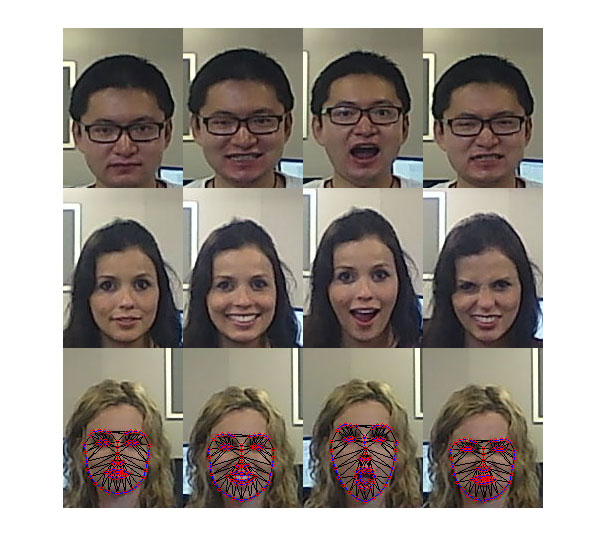
\includegraphics[width=0.95\textwidth,height=70mm]{figures/dataExtrationExamples.jpg}
\end{center}
\caption{\textbf{Data extraction} Samples of the face shapes recorded.}
\label{figureLabel}
\end{figure}

For every face shape recorded, it was taken 20 samples with a small time
interval between them (less than one second). Each sample consists on the record
of the invariant vector that transforms a neutral face shape into the deformed
face shape that fits the subject. Since there was fuctiations on the borders
of the face shape recognizer and thus generating some instabililty on the
invariant vector, it's was taken 20 samples to minimize this error.

During the data extraction period, it was seen that every person has a unique
invariant vector, and it was tought that it could be used to recognize people
aswell. This event can be seen in the Figure ?.

On recognizing face expression, even though every person has its own unique
features vector for each face expression, there is a similarity between these vectors when comparing
the same face shape of different people, thus the goal of the SVM was to
generate an abstraction of what is this face shape and to become able to identify face expressions.

\subsubsection{Data training}

For data training the testing, it was used a 10-fold cross validation on every
sector. 



\begin{figure}[ht]
\begin{center}
\vspace{-3mm}
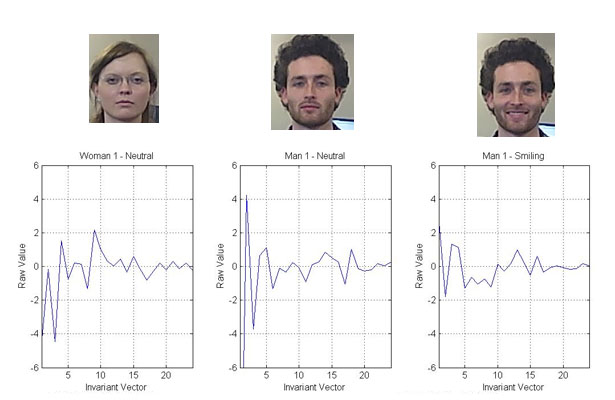
\includegraphics[width=0.95\textwidth,height=70mm]{figures/comparationBetweenFaces.jpg}
\end{center}
\caption{\textbf{People representation} The diferences of the invariant
vector from differents face shapes and people.}
\label{figureLabel}
\end{figure}

a
\section{Results}
The results of the identity recognition experiments are shown in Figure \ref{}.

In this section, it will be shown the results of three on three different
approachs, on recognizing face expressions, recognizining face expressions using
different number of classes and recognizing people.

\subsection{Recognizing Face Expressions}

In this approach, the goal was to recognize each of the 11 different classes, it
was used a 10-fold cross validation to measure the perfomance of
 the SVM algorithm. It was used all the 24 features of each face shape. It was
 given two differents aproach on the performance measurement. The first one was
 by separating the 20 samples of each person face expression into two segments,
 one containing 17 samples and other 3. The 17 samples were used to train while
 the remaining ones to test. This approach will be called Including. The second
 approach was by using all the 20 samples but using different people one the
 training set and the testing set. It was kept the same ratio for the second
 approach, 70\%.
 
\begin{figure}[ht]
\begin{center}
\vspace{-3mm}
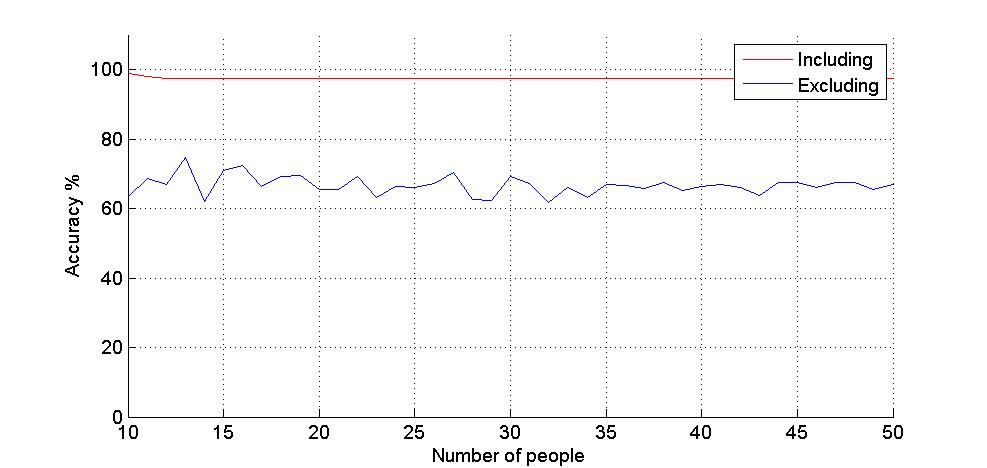
\includegraphics[width=0.95\textwidth,height=50mm]{figures/figureRecognizeFacialExpression.jpg}
\end{center}
\caption{\textbf{Identity Recognition Results} Explanation of the figure.}
\label{identityRecognition}
\end{figure}

The results of the facial expression recognition  are shown in Figure
\ref{identityRecognition}.
 
\subsection{Recognizing Face Expressions increasing the number of classes}

Using a 10-fold cross validation, in this approach the goal was to measure the
change of effiency of the algorithm by increasing the number of classes from 2
to 11. The amount of people used was 50.

\begin{figure}[ht]
\begin{center}
\vspace{-3mm}
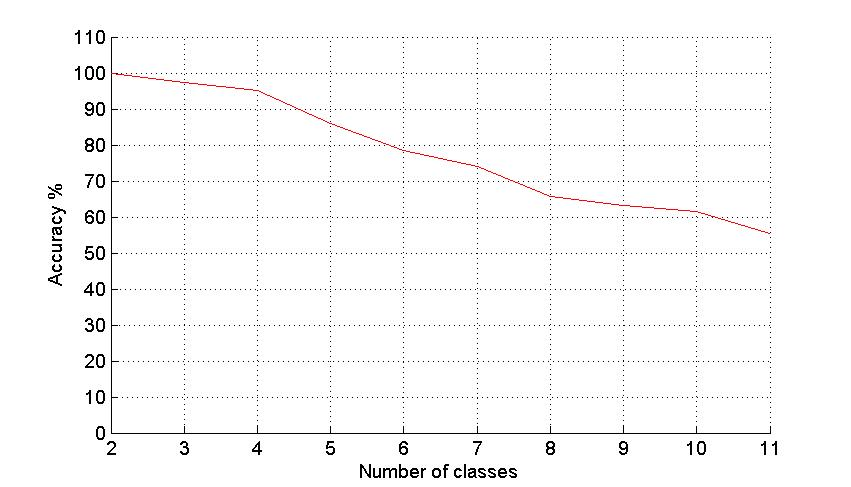
\includegraphics[width=0.95\textwidth,height=50mm]{figures/50people_increasing_classes.jpg}
\end{center}
\caption{\textbf{Effect of Increasing the Number of Facial Expressions to Recognize} Explanation of the figure.}
\label{increasingNumberExpressions}
\end{figure}

Figure \ref{feRecognition} shows the results of increasing the number of people
to be recognized by the classifier.

\subsection{Recognizing People}

In the third approach, there is a change on what are the classes of the
algorithm. Instead of face shapes being the classes, in this method, the people
to recognize were transformed into the classes. Therefore, the increase of
people to recognize increase the number of the classes, thus decreasing the
efectiviness of the algorithm. It was analysed from 2 to 50 people the algorithm
accuracy. It was also analysed in three different scenarios, using only the
normal face shape, using only 6 and using all 11 face shapes in each classe.
 


\begin{figure}[ht]
\begin{center}
\vspace{-3mm}
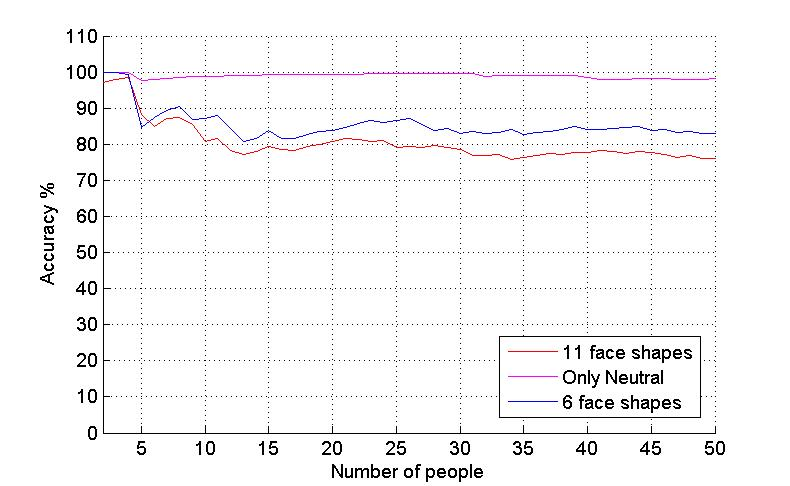
\includegraphics[width=0.95\textwidth,height=50mm]{figures/peopleRecognition.jpg}
\end{center}
\caption{\textbf{Facial Expression Recognition Results} Explanation of the figure.}
\label{feRecognition}
\end{figure}


Figure \ref{feRecognition} shows the results of increasing the number of people
to recognize facial expressions


\section{Discussion}
In this work we have used an open-source face tracker to recognize facial identity and to classify facial expressions.


\bibliographystyle{plain}
\bibliography{library}

\end{document}
